\chapter{Arkitektur}

Arkitekturafsnittet i denne del af dokumentationen vil være inddelt efter widgets og overordnet funktionalitet i applikationen. Det vil sige at for hvert hoved funktionalitet i applikationen er der udarbejdet en arkitektur, der med brug af UML og anden strukturel visualisering, giver en god indsigt i hvordan WePlanner er struktureret og hvordan de forskellige iterationer har været. Desuden har arkitekturen hele tiden været under udvikling - flere iterationer. Da projektet er blevet udviklet i sprints af 2 uger ad gangen, er arkitekturen også udviklet i 2 uger ad gangen.

\section{1. Iteration}

Som med mange projekter, kræver det en del tid at komme rigtigt i gang. Denne iteration blev brugt meget på at skabe overblik og fælles forståelse for hvad projektet skulle bestå af. Fra undervisningen i GUI, blev MVC introduceret og der blev givet følgende model\cite{mvcControllerModel}:
\begin{figure}[hbt]
    \centering
    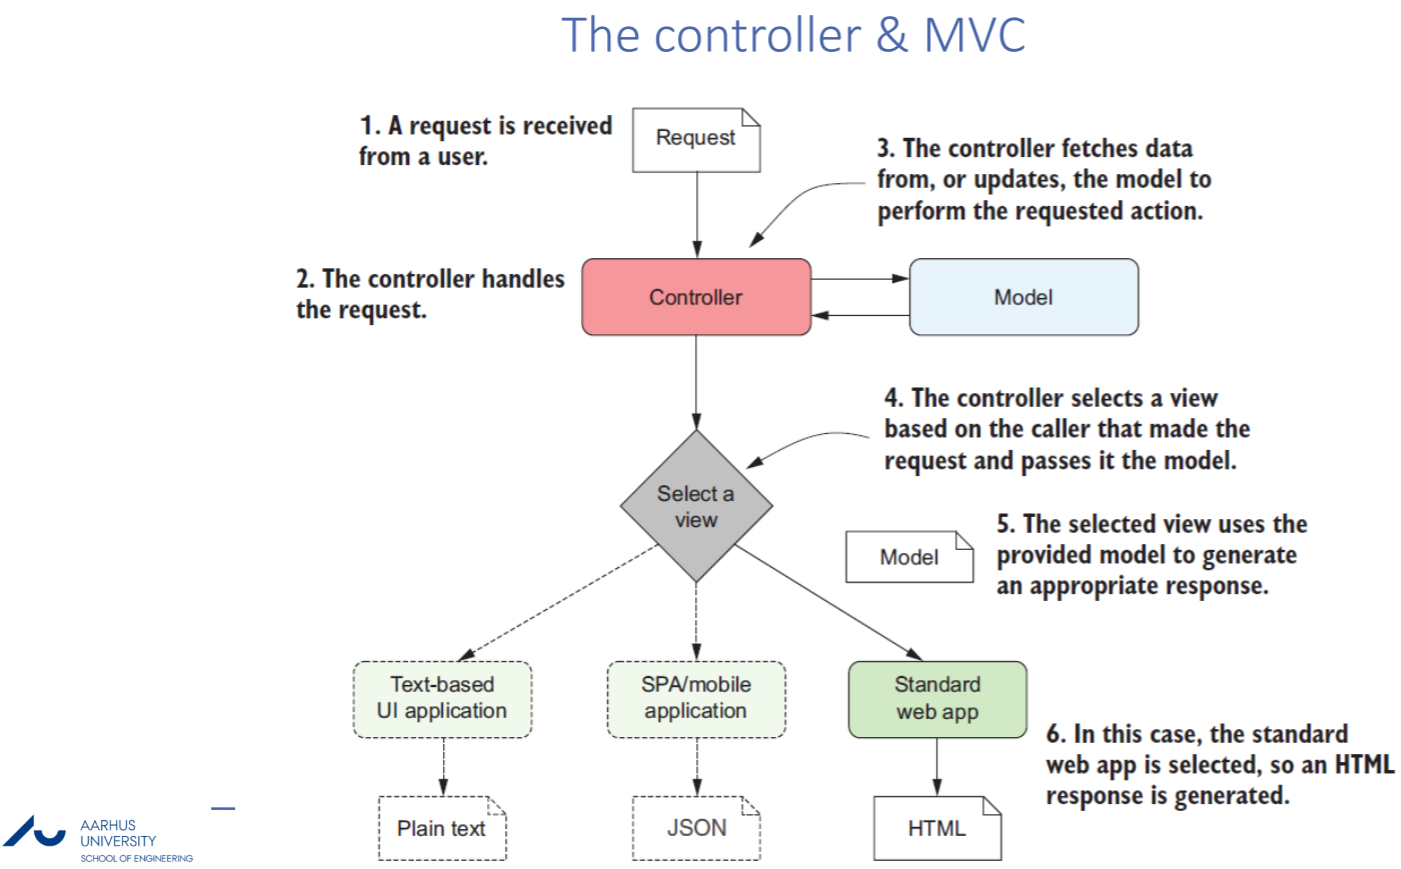
\includegraphics[scale=0.5]{Images/Arkitektur/MVC_Controller.png}
    \caption{Controllers rolle i MVC}
    \label{fig:MVC_Controller}
\end{figure}

Denne model beskriver meget præcist hvordan hele webapplikationen ift. MVC kommer til at hænge sammen.






\section{2. Iteration}

\subsection{ASP.NET Framework MVC}